\chapter{Aufnahme von Koordinatenpunkte}
\section{Problem}
Wenn ein Koordinatenpunkt aufgenommen werden will, gibt es mehrere Probleme auf die man stößt.

Zum einen kann man nicht zur gleichen Zeit die X und Y Komponente der Koordinate bestimmen, dies muss nacheinander folgen.
Grund hierfür ist dem Aufbau des Touchscreens geschuldet.

Bei der Inbetriebnahme wird sich noch ein weiteres Problem ergeben.
Falls der Touchscreen nicht betätigt wird, gibt der Mikrocontroller trotzdem Werte aus.
Dabei handelt es sich um Werte die keinen Sinn ergeben und die Steuerung der Maus z.B. bei einer Ruhephase stören würden.

Wenn Werte aufgenommen werden kann es vorkommen, dass diese vereinzelte Sprünge aufweißen oder keine fließende Führung auf dem Touchscreen nachempfinden.
Dieses Problem ist der Messunsicherheit des Systems geschuldet, die es zu  minimieren gilt.

\section{Lösungsansatz}
Um das Problem, bei einer nicht Betätigung des Touchscreens, zu lösen soll vor einer Aufnahme von Koordinatenwerte geprüft werden, ob der Touchscreen betätigt wird.
Ist dies der Fall so soll die Messung durchgeführt werden.

Um eine Koordinatenkomponente zu bestimmen, benötigt man drei Anschlüsse des Touchscreens.
Zwei davon sind in der Richtung die man messen möchte und der dritte Anschluss ist einer der beiden übrigen Anschlüsse.
Mit diesem wird der Spannungsteiler auf gespannt um den Wert der Koordinate zu bestimmen.

In den Abbildungen \cref{fig:xylesen} auf Seite \cref{fig:xylesen} wird dieser Lösungsansatz veranschaulicht.
Bei dem Lesen der x-Komponente \cref{fig:xlesen} wird der Pin \verb$X_Le$ (steht für X-Links) auf eine Spannung von \SI{5}{V} gesetzt.
Der Pin \verb$X_Ri$ (steht für X-Rechts) wird auf \SI{0}{V} gezogen.
Der Pin  \verb$Y_Up$ (steht für Y-Oben) wird der ADC angeschlussen, sodass dieser Pin für das auslesen der Werte des Spannungsteiler sind.
Um die y-Komponente zu lesen wird das wie in Abbildung \cref{fig:ylesen} auf Seite \cref{fig:ylesen} der Pin \verb$Y_Up$ auf \SI{5}{V} gesetzt und der Pin \verb$Y_Lo$ (steht für Y-Unten) auf \SI{0}{V} gesetzt.
Der ADC misst über den Pin \verb$X_Le$.

Die Pins die bei der Messung nicht miteinbezogen sind, werden in den jeweiligen Schaltungen deaktiviert.

Um nun noch eine Messunsicherheiten aus zu filtern sollen, bei der Messung einer Koordinatenkomponente, mehrere Messpunkte aufgenommen werden.
Diese werden anschließend über ein Filter-Funktion ausgewertet.
Der Wert der bei der Auswertung als Ergebnis herrauskommt, wird als gemessene Koordinatenkomponente ausgegeben.
Die jeweiligen Pins die mittels des ADC die Messung durchführen werden bei der Messung an einen PullUp Widerstand angeschlossen.
Somit ist der Wiederstander von \verb$R_yup$ (für die x-Komponente) und \verb$R_xle$ (für die y-Komponente) vernachlässigbar gering und tärgt zum Messergebnis eine vernachläsigbaren Beitrag hinzu.
Das Schaltbild hier zu ist in Abbildung \cref{fig:schaltbild} zu sehen.

\begin{figure}[ht!]
    \begin{subfigure}{0.49\textwidth}
        \centering
        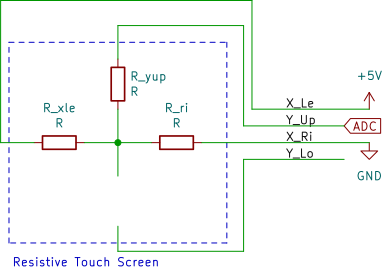
\includegraphics[width=\textwidth]{fig/xlesen.png}
        \caption{in x-Richtung}
        \label{fig:xlesen}
    \end{subfigure}
    \hfill
    \begin{subfigure}{0.49\textwidth}
        \centering
        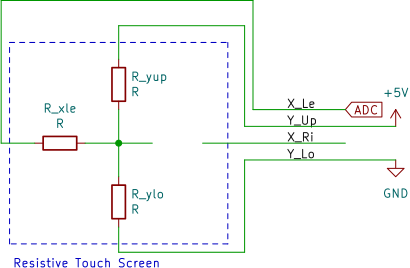
\includegraphics[width=\textwidth]{fig/ylesen.png}
        \caption{in y-Richtung}
        \label{fig:ylesen}
    \end{subfigure}
    \caption{Schaltbild für das Messen der Koordinatenpunkte}
    \label{fig:xylesen}
\end{figure}
\begin{figure}[ht!]
    \centering
    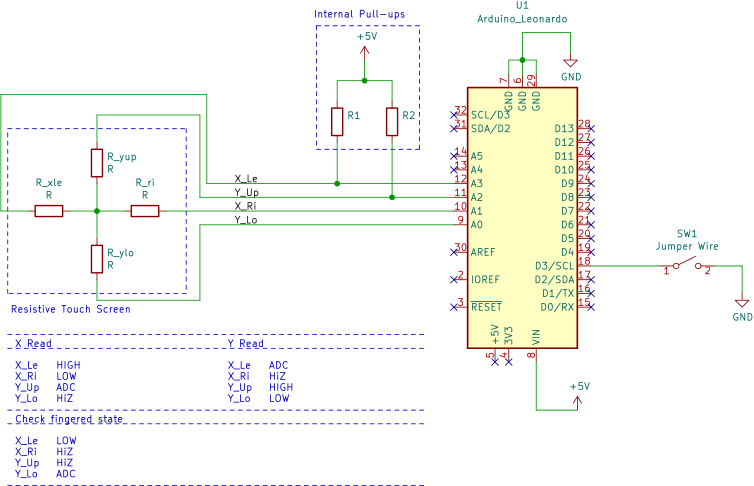
\includegraphics[width=\linewidth]{fig/schaltbild.png}
    \caption{Schaltbild des Projekts}
    \label{fig:schaltbild}
\end{figure}
Die einzelne Lösungsansätze werden in der Arduino-Umgebung umgesetzt.
Der Programmablauf ist in \cref{fig:flowchart} als Flow-Chart dargestellt.

\begin{figure}
    \centering
    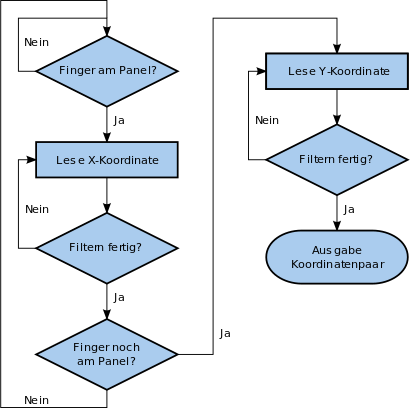
\includegraphics[scale=0.45]{fig/flow_chart.png}
    \caption{Darstellung des Programmablaufs}
    \label{fig:flowchart}
\end{figure}
\section{Umsetzung des Lösungsansatz}
\section{Filterung der Messpunkte}